\documentclass{beamer}
%\documentclass[17pt]{beamer}
%**********************************************************************************************************************************************
\usepackage{multicol, stmaryrd, amsfonts, graphicx, times, epsfig, amsmath, mathtools, subfigure, balance, array, siunitx, pgfgantt, xspace}
\usepackage{multirow, epsf, amsmath, amssymb, indentfirst, verbatim, keyval, url, textcomp, enumerate, calc, makecell, subfigure, xcolor, listings}
%**********************************************************************************************************************************************
\usepackage[utf8]{inputenc}
\usepackage[export]{adjustbox}
\usepackage[absolute,overlay]{textpos}
\usepackage{hyperref}
\usepackage[normalem]{ulem}
\usepackage{textpos}
\usepackage{tcolorbox}
%**********************************************************************************************************************************************
\useunder{\uline}{\ulined}{}%
\DeclareUrlCommand{\bulurl}{\def\UrlFont{\ttfamily\color{blue}\ulined}}
\usefonttheme{serif}
\usetheme{Pittsburgh}
\usecolortheme{beaver}
\graphicspath{ {figs/} }
\setbeamertemplate{itemize items}[ball]
\setbeamertemplate{bibliography item}[text]
\hypersetup{
   colorlinks   = true,                               %Colours links instead of ugly boxes
   urlcolor     = blue,                               %Colour for external hyper links
   linkcolor    = blue,                               %Colour of internal links
   citecolor    = red,                                %Colour of citations
   setpagesize  = false,
   linktocpage  = true,
}
%**********************************************************************************************************************************************
%\usepackage{stmaryrd, amsfonts, graphicx, times, epsfig, amsmath, mathtools,subfigure, balance, array,siunitx}
%\usefonttheme{structuresmallcapsserif}
%\usepackage{bookman}
%\usetheme{Madrid}
%\usetheme{Szeged}
%**********************************************************************************************************************************************
 \AtBeginSection[]
{
  \begin{frame}
    \frametitle{Table of Contents}
    \tableofcontents[currentsection]
  \end{frame}
}
%**********************************************************************************************************************************************
%Information to be included in the title page:
\title[] %optional
{Graph Neural Network \\Lecture 1}
%\subtitle{Graph Neural Network \\Lecture}
%**********************************************************************************************************************************************
%\author[Arthur, Doe] % (optional, for multiple authors)
%{A.~B.~Arthur\inst{1} \and J.~Doe\inst{2}}
%
%\institute[VFU] % (optional)
%{
%  \inst{1}%
%  Faculty of Physics\\
%  Very Famous University
%  \and
%  \inst{2}%
%  Faculty of Chemistry\\
%  Very Famous University
%}
%**********************************************************************************************************************************************
\date[] % (optional)

%\logo{\includegraphics[width=1in, height=0.3in]{GW_logo.eps}}
\titlegraphic{
\includegraphics[width=0.8in, height=0.8in]{FrontCover_ImgID1_mod3.eps}}
%>>>>>>>>>>>>>>>>>>>>>>>>>>>>>>>>>>>>>>>>>>>>>>>>>>>>>>>>>>>>>>>>>>>>>>>>>>>>>>>>>>>>>>>>>>>>>>>>>>>>>>>>>>>>>>>>>>>>>>>>>>>>>>>>>>>>>>>>>>>>>>>
%>>>>>>>>>>>>>>>>>>>>>>>>>>>>>>>>>>>>>>>>>>>>>>>>>>>>>>>>>>>>>>>>>>>>>>>>>>>>>>>>>>>>>>>>>>>>>>>>>>>>>>>>>>>>>>>>>>>>>>>>>>>>>>>>>>>>>>>>>>>>>>>


\begin{document}

\begin{frame}
    % Print the title page as the first slide
    \titlepage
\end{frame}

\begin{frame}{Overview}
    % Throughout your presentation, if you choose to use \section{} and \subsection{} commands, these will automatically be printed on this slide as an overview of your presentation
    \tableofcontents
\end{frame}

%------------------------------------------------
\section{Introduction to GNNs}
%------------------------------------------------

\begin{frame}{What Are Graph Neural Networks?}
    \begin{itemize}
        \item GNNs are a type of deep learning model designed for graph-structured data
        \item Graphs consist of:
                \begin{itemize}
                \item Nodes (Vertices): Represent entities (e.g., people in a social network).
                \item Edges/Links: Represent relationships or interactions (e.g., friendships).
                
                \vspace{0.3cm}
                \centering % Center the TikZ picture
                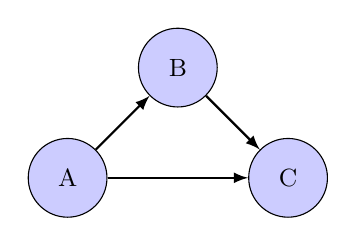
\begin{tikzpicture}[
                    node/.style={circle, draw=black, fill=blue!20, minimum size=1cm, font=\small},
                    edge/.style={->, >=latex, thick}
                ]
                \begin{scope}[scale=0.7] % Scale down the entire diagram
                    % Nodes
                    \node[node] (A) at (0, 0) {A};
                    \node[node] (B) at (2, 2) {B};
                    \node[node] (C) at (4, 0) {C};
    
                    % Edges
                    \draw[edge] (A) -- (B);
                    \draw[edge] (B) -- (C);
                    \draw[edge] (A) -- (C);
                    % Labels
                    % \node[below=0.7cm of A] {Node features};
                \end{scope}
                \end{tikzpicture}
                \end{itemize}
        \item GNNs leverage the structure of graphs to learn meaningful representations.   
    \end{itemize}
    
\end{frame}

%------------------------------------------------
\begin{frame}{Key Components of GNNs}
    \begin{block}{Message Passing:}
        Nodes aggregate information from neighbors.
    \end{block}

    \begin{block}{Node Embeddings}
        Transform features into a low-dimensional vector space.
    \end{block}

    \begin{block}{Graph Aggregation:}
        Pool node embeddings to form a graph-level representation.
    \end{block}
    
\end{frame}

%------------------------------------------------
\begin{frame}{Why Use GNNs?}
    \begin{itemize}
        \item Graph data is everywhere in real-world applications.
        \item Traditional neural networks struggle with non-Euclidean data.
        \item GNNs enable learning directly on graph structures, capturing both:
        \begin{itemize}
            \item Node features.
            \item Topological relationships (connectivity).
        \end{itemize}
    \end{itemize}
\end{frame}

%------------------------------------------------
\begin{frame}{Examples of Graph Data}
    \begin{itemize}
        \item Social networks: Users as nodes, friendships as edges.
        \item Molecular graphs: Atoms as nodes, chemical bonds as edges.
        \item Knowledge graphs: Entities as nodes, relationships as edges.
        \item Transportation networks: Locations as nodes, roads as edges.
    \end{itemize}
\end{frame}

\section{Key Concepts of GNNs}

%------------------------------------------------
\begin{frame}{Architecture Overview}
    \begin{itemize}
        \item General structure:
        \begin{itemize}
            \item \textbf{Input:} Graph data (nodes, edges, and features).
            \item \textbf{Hidden layers:} Message passing and aggregation.
            \item \textbf{Output:} Node embeddings, edge predictions, or graph-level classifications.
        \end{itemize}
        \item Iterative information exchange across graph layers.
        \item Key insight: Combining node features with graph topology.
    \end{itemize}
\end{frame}

%------------------------------------------------
\begin{frame}{GNN Workflow}
    \begin{enumerate}
        \item Initialize node features (e.g., feature vectors).
        \item Perform message passing for multiple layers.
        \item Aggregate and update node embeddings.
        \item Apply task-specific layers (e.g., classification or regression).
    \end{enumerate}
\end{frame}

%------------------------------------------------
\section{Applications of GNNs}
%------------------------------------------------
\begin{frame}{Applications of GNNs}
    \begin{itemize}
        \item \textbf{Social Networks:} Friend recommendation, community detection.
        \item \textbf{Knowledge Graphs:} Entity linking, relation prediction.
        \item \textbf{Drug Discovery:} Molecular property prediction.
        \item \textbf{Transportation:} Traffic forecasting, route optimization.
    \end{itemize}
\end{frame}

%------------------------------------------------
\begin{frame}{Advantages and Challenges}
    \begin{columns}
        \column{0.5\textwidth}
        \textbf{Advantages:}
        \begin{itemize}
            \item Captures graph topology.
            \item Flexible and powerful.
            \item Handles irregular data.
        \end{itemize}

        \column{0.5\textwidth}
        \textbf{Challenges:}
        \begin{itemize}
            \item Computationally expensive.
            \item Scalability to large graphs.
            \item Over-smoothing in deep GNNs.
        \end{itemize}
    \end{columns}
\end{frame}

%------------------------------------------------
\section{Summary}
%------------------------------------------------
\begin{frame}{Summary}
    \begin{itemize}
        \item Graph Neural Networks generalize deep learning to graph-structured data.
        \item Applications span diverse domains such as social networks, biology, and recommendation systems.
        \item Ongoing research addresses scalability and optimization challenges.
    \end{itemize}
\end{frame}
%------------------------------------------------


%------------------------------------------------

%------------------------------------------------

%------------------------------------------------



%------------------------------------------------

% \begin{frame}[fragile] % Need to use the fragile option when verbatim is used in the slide
%     \frametitle{Citation}
%     An example of the \verb|\cite| command to cite within the presentation:\\~

%     This statement requires citation \cite{p1}.
% \end{frame}

%------------------------------------------------

% \begin{frame}{References}
%     \footnotesize
%     \bibliography{reference.bib}
%     \bibliographystyle{apalike}
% \end{frame}



%----------------------------------------------------------------------------------------

\end{document}